
\title{Lab Report 11 - Condensation Tracker}
\author{
        Manuel Galliker  14-921-969 \\
                manuelga@student.ethz.ch
}
\date{\today}

\documentclass[12pt]{article}
\usepackage{graphicx}
\usepackage{float}
\begin{document}
\maketitle


\section{Implementation }

The algorithm was implemented as described in the exercise sheet. The functions for the colour histogram, propagation, observation, estimation and resampling were implemented according to they're formulas. This time the explanation was well done and is pretty complete.
\newline
For the $A$ matrix the following configurations were choosen:
\newline 
\vspace{5mm}
No motion model: 

$ A = \left[ \begin{array}{rrrr}
1  & 0 \\
0 &  1 \\
\end{array}\right] $
\vspace{5mm}
\newline
$particles = A*particles + n_{pos}$

\vspace{5mm}

Constant motion model:
\vspace{5mm}
\newline
$ A = \left[ \begin{array}{rrrr}
1 & 0 & 1 & 0 \\
0 & 1 & 0 & 1 \\
0 & 0 & 1 & 0 \\
0 & 0 & 0 & 1 \\
\end{array}\right] $
\vspace{5mm}
\newline
$particles = A*particles +  \left[ \begin{array}{rrrr}
n_{pos} \\
n_{vel} \\
\end{array}\right]$

\section{Video 1}

Video 1 shows a moving hand in front of a uniform background. As can be seen the horizontal position of the hand is tracked quite well. But the vertical tracking performs significantly worse. This might be due to the motion blur making the finger tips brighter, which shiftes the colour histogram. In that case the histogram of a box lower in the arm fits the original one better.


\vspace{5mm}
\begin{figure}[H]
	\centering
	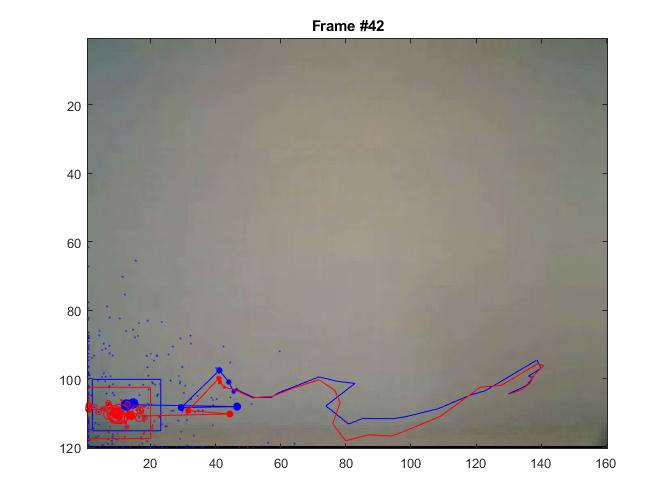
\includegraphics[width=0.9\textwidth]{1.jpg}
	\caption{Trajectories for video 1 with standart parameters}
	\label{fig1}
\end{figure}
\vspace{5mm}

\section{Video 2}

\subsection{Model Choice}
Video 2 shows a moving hand with some clutter and occlusion. First the const. position and velocity models are tested. 


\vspace{5mm}
\begin{figure}[H]
	\centering
	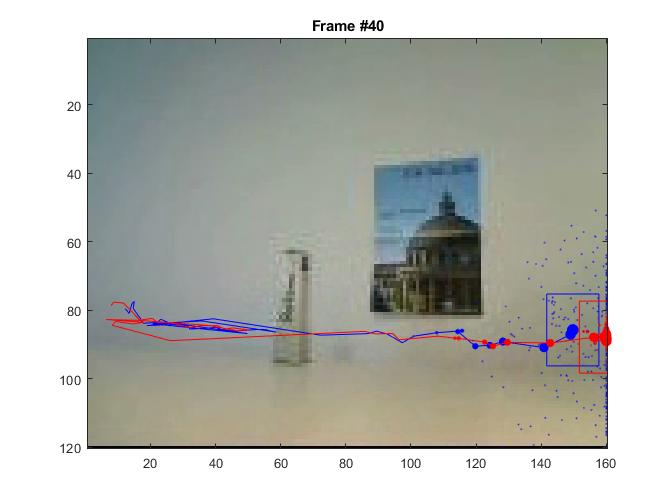
\includegraphics[width=0.9\textwidth]{bad_position_model.jpg}
	\caption{Const. position model}
	\label{fig1}
\end{figure}
\vspace{5mm}
\vspace{5mm}
\begin{figure}[H]
	\centering
	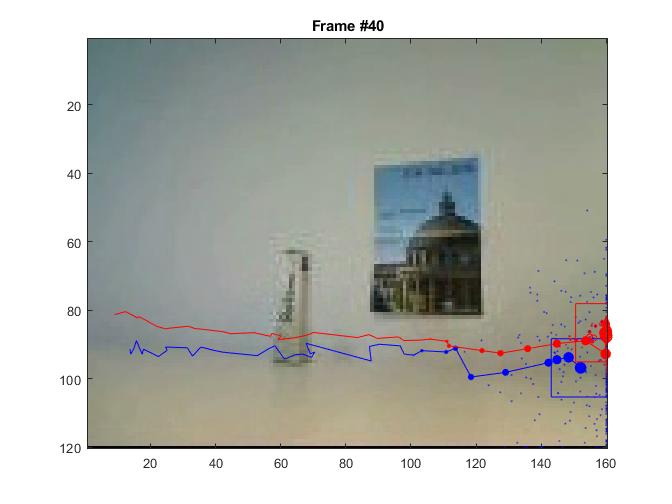
\includegraphics[width=0.9\textwidth]{const_vel.jpg}
	\caption{Const. velocity model}
	\label{fig1}
\end{figure}
\vspace{5mm}

The const velocity model performs way better when the object is occluded, which makes intuitively a lot of sense since the constant velocity assumption helps to search in the generral direction of the hand. 
Furthermore, with the const. velocity model the a priori mean state lies generally distinctively lower than the posteriori mean state due to the initial velocity estimate. more on that later. Simillar to the situation before the horizontal position of the hand is tracked better due to the same reason. 

\subsection{System noise}
\vspace{5mm}
\begin{figure}[H]
	\centering
	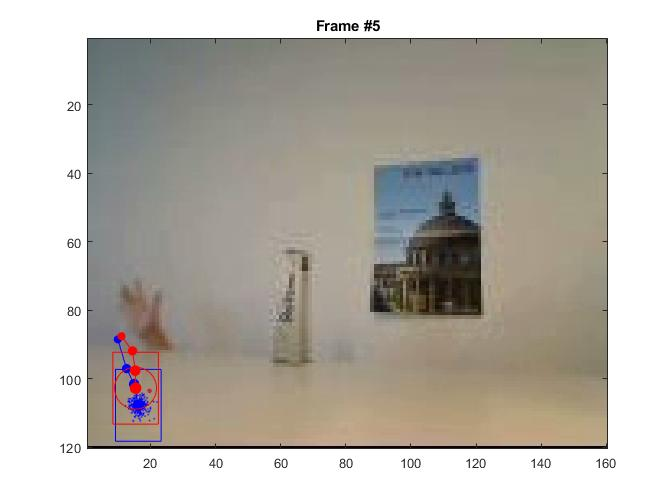
\includegraphics[width=0.9\textwidth]{low_noise.jpg}
	\caption{low system noise: $\sigma_p = 1.5$, $\sigma_v = 0.1$}
	\label{fig1}
\end{figure}
\vspace{5mm}
the point distribution is not spread sufficiently large enough to track the hand. This leads to a failure in tracking. The system noise should be choosen suffently large but not too large. 
\vspace{5mm}
\begin{figure}[H]
	\centering
	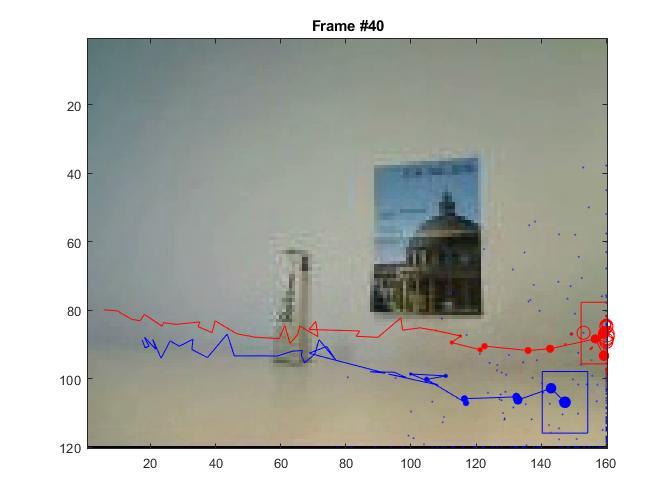
\includegraphics[width=0.9\textwidth]{high_noise.jpg}
	\caption{high system noise: $\sigma_p = 30$, $\sigma_v = 2$}
	\label{fig1}
\end{figure}
\vspace{5mm}
With the above parameters the noise is slightly too high which leads to less points landing on the hand and a more noisy tracking line. 
\vspace{5mm}
\begin{figure}[H]
	\centering
	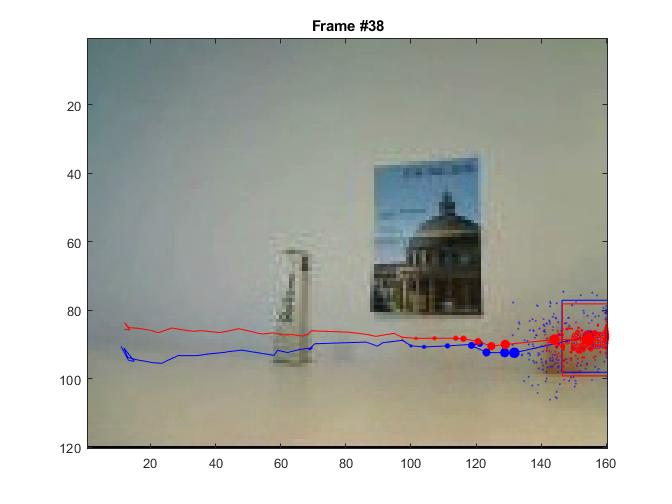
\includegraphics[width=0.9\textwidth]{normal_low_noise.jpg}
	\caption{good system noise: $\sigma_p = 7.5$, $\sigma_v = 0.5$}
	\label{fig1}
\end{figure}
This results in better and more smooth tracking of the hand and this was choosen as the best parameter set for the system noise. Furthermore it should be noted, that the const. velocity model allowes for a smaller system noise to be choosen and therefore results in a better tracking as well.
\begin{figure}[H]
	\centering
	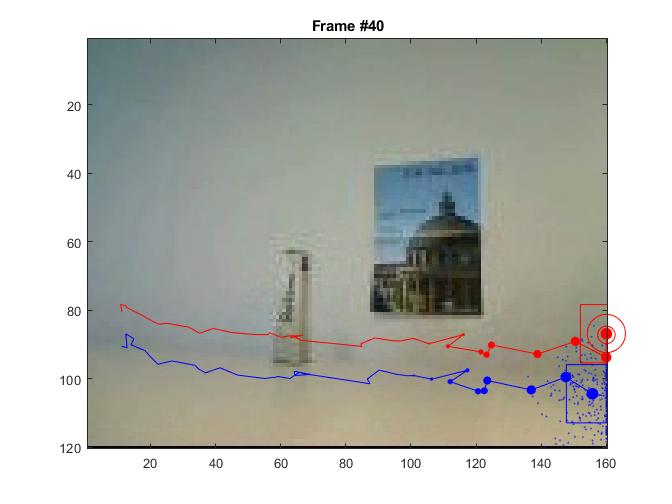
\includegraphics[width=0.45\textwidth]{observe_002.jpg}
	\caption{low measurement noise: $\sigma_m = 0.02$}
	\label{fig1}
\end{figure}
\begin{figure}[H]
	\centering
	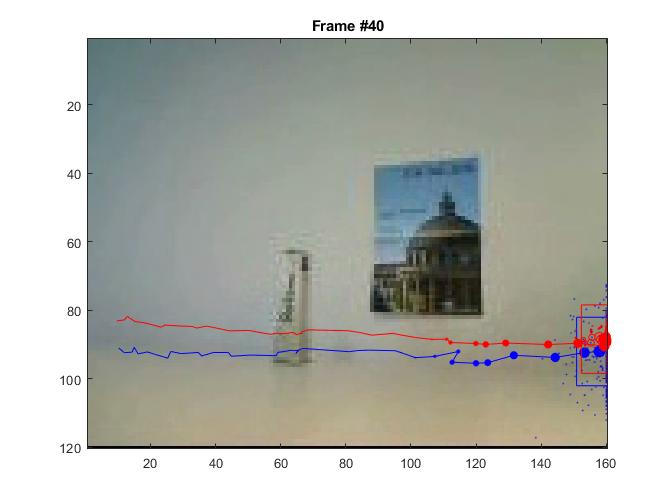
\includegraphics[width=0.45\textwidth]{observe_normal.jpg}
	\caption{good measurement noise: $\sigma_m = 0.1$}
	\label{fig1}
\end{figure}
\begin{figure}[H]
	\centering
	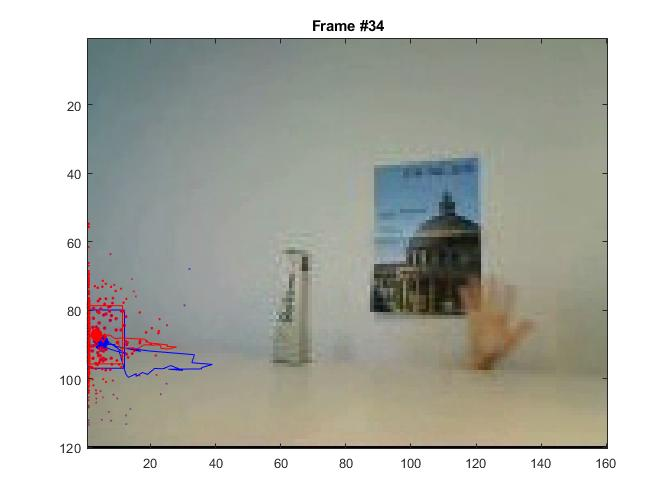
\includegraphics[width=0.45\textwidth]{observe_05.jpg}
	\caption{high system noise: $\sigma_m = 0.5$}
	\label{fig1}
\end{figure}
As can bee seen a too high system noise can lead to loosing the object that should be tracked. The best result was achieved in the image in the middle and this parameter choice was kept. 
\newline
The provided initial velocity was performing already quite well. But it was still slightly adapted:
\begin{figure}[H]
	\centering
	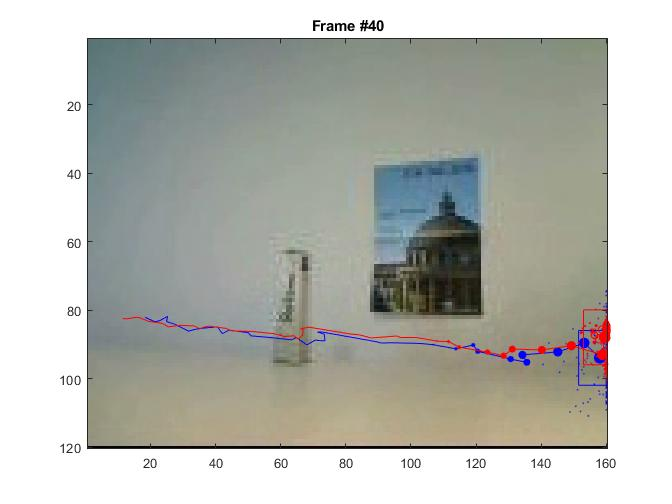
\includegraphics[width=0.9\textwidth]{v-1.jpg}
	\caption{good initial velocity: $v_x = 10$, $v_y=1$}
	\label{fig1}
\end{figure}


\section{Video 3}
\begin{figure}[H]
	\centering
	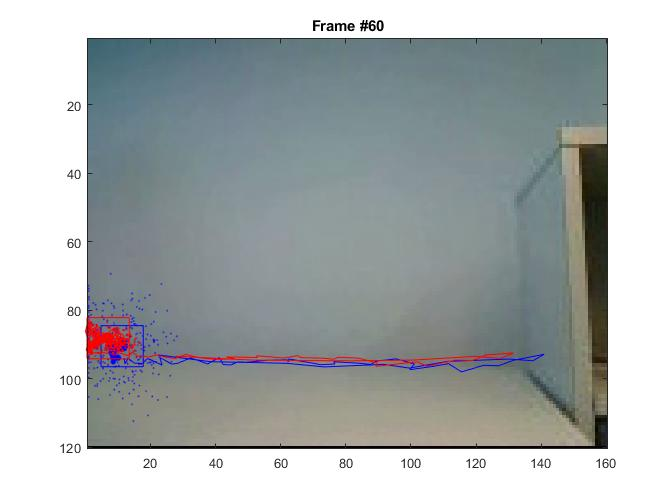
\includegraphics[width=0.9\textwidth]{vid3.jpg}
	\caption{Tracking of the ball in video 3}
	\label{fig1}
\end{figure}
Here, the tracking works very well out of the box. Since the full object is visible in frame one and the colour and brightness contrast to the background is way more drastic the tracking is way easier in this example. So while exact parameter tuning could still make the tracking curve somewhat smoother it is not as critical here as in video 2. Important however is, that the spreading of the points is sufficiently large to still include the ball after bouncing from the wall. 


\section{Discussion}
\subsection{particle number}
More particles is generally good with a well tuned spread since it allows a more exact tracking. This is however computationally more expensive and follows the law of diminishing returns. After a certain point though more points will just lead to tracking noise instead of the actual movement. 
\subsection{bin number}
A higher bin number is required when the color and brightness contrass between object and background is smaller. 
\subsection{appearance model updating}
This allowes the histogram to be adjusted over time. Generally this is very usefull for sudden brightness or color variations but can also lead to a misclassification of the object for example when its occluded and $\alpha$ is too high. 
\begin{figure}[H]
	\centering
	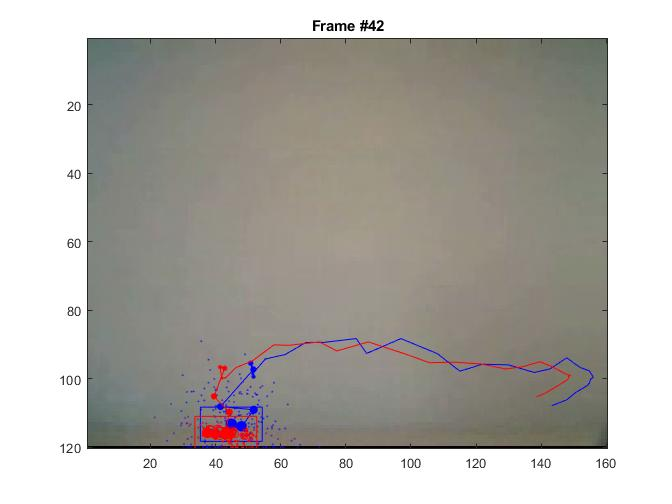
\includegraphics[width=0.9\textwidth]{vid1_2.jpg}
	\caption{Video 1 with final parameter choice and $\alpha = 0.2$}
	\label{fig1}
\end{figure}
\begin{figure}[H]
	\centering
	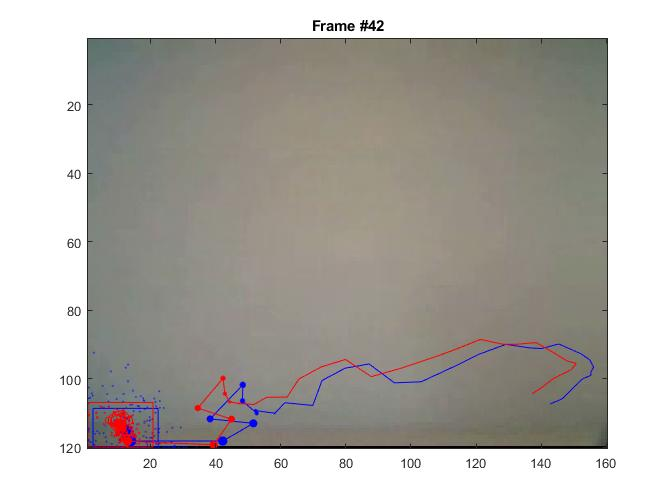
\includegraphics[width=0.9\textwidth]{vid_1_3.jpg}
	\caption{Video 1 with final parameter choice and $\alpha = 0$}
	\label{fig1}
\end{figure}
As can be seen this is a very good strategy when there is little or no clutters and the background is therefore clearly destincteable from the object.
\vspace{5mm}
\newline

Last but not least i wish you a merry christmas and a happy new year! 
\end{document}

